\section{Cluster-based Map Abstraction}
\label{aha:mapabstraction}
AA* is sufficient for low-level planning on the original gridmap but inefficient for large problem sizes; we would prefer to express a more general strategy using macro-operators.
Our result from theorem {\ref{aha-theorem:reducibility} is key to the spatial abstraction described in this section. 
\par \indent
We extend the process in \cite{botea04} which involves dividing a grid map into fixed-size square sections called \emph{clusters}. 
Figure \ref{aha-fig:clustersandentrances}(a) shows the result of this decomposition approach; we use clusters of size 5 to split our toy map into 4 adjacent sections. 
\par \indent
In the original work \emph{entrances} are defined as obstacle-free transition areas of maximal size that exist along the border between two adjacent clusters.
Each entrance has one or two transition points (depending on its size) which are represented in the abstract graph by a pair of nodes connected with an undirected \emph{inter-edge} of weight 1.0. 
We use a similar approach but require as a parameter $C$, the set of all capabilities, and thus attempt to identify entrances for each $c \in C$. 
\begin{figure}[htbp]
	\vspace{-15pt}
        \caption{\emph{Building clusters and identifying entrances} }
        \begin{center}
                        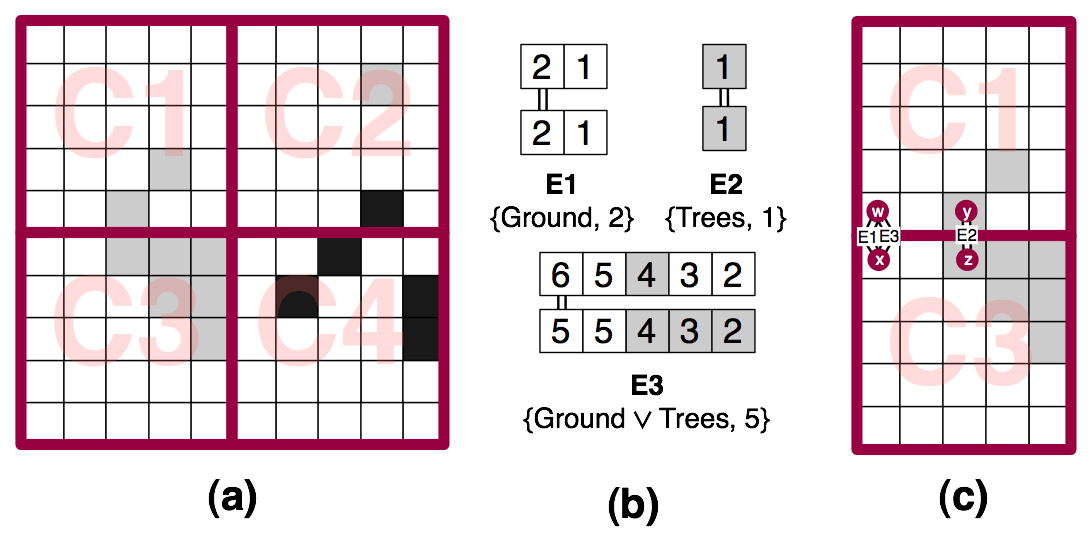
\includegraphics[scale=0.30, trim = 20mm 12mm 20mm 5mm]{diagrams/identifying_entrances.png}
        \end{center}
        \label{aha-fig:clustersandentrances}
	\vspace{-6pt}
\end{figure}
\par \indent
We start at the first pair of traversable tiles along the adjacent border area and extend each entrance until one of three termination conditions occurs: the end of the border area is reached, an obstacle is detected or the clearance value of nodes along the border area in either cluster begins to increase. 
The last condition is important to preserve representational completeness for large agents in cases where a cluster is partially divided by an obstacle (such as a wall) near the border.
By leveraging clearance we are able to reason about the presence of such obstacles and build a new entrance each time we detect the amount of traversable space inside either cluster is increasing.
\par \indent
Once an entrance is found, we choose as the transition point the first pair of adjacent nodes in each cluster which maximise clearance for $c$.
This latter metric, $cv_{inter}$ is computed by taking the minimum clearance among each pair of adjacent nodes in the entrance area and selecting the largest value from the set. 
Thus, we add a new edge to the graph, $e_{inter}$ and annotate it with a single capability and corresponding clearance value, $e_{inter}(c) = cv_{inter}$. 
The algorithm repeats for each $c \in C$ and terminates when all adjacent clusters have been considered. 
This ensures we identify all possible entrances for each available capability.
\par \indent
In Figure \ref{aha-fig:clustersandentrances}(b) we present three entrances identified by scanning the border between clusters $C1$ and $C3$.
Entrances \emph{E1} and \emph{E2}, each of which span only part of the border area, are discovered using the $\lbrace Ground \rbrace$ and $\lbrace Trees \rbrace$ capabilities respectively. 
\emph{E3} meanwhile, which spans the whole border area, is discovered using the $\lbrace Ground \vee Trees \rbrace$ capability. 
The connected tiles represent the locations of the subsequent transition points; the final result is shown in Figure \ref{aha-fig:clustersandentrances}(c). 
Note that \emph{E1} and \emph{E3} are incident on the same pair of nodes in the abstract graph. This is due to our  strategy of actively attempting to re-use any existing nodes from the abstract graph. 
\par \indent
The final step in the decomposition involves attempting to add to the abstract graph a set of \emph{intra-edges} for each pair of abstract nodes inside a cluster. 
We achieve this by running multiple AA* searches $\forall (c, s) : c \in C, s \in S$.
Once a path is found we annotate the new edge, $e_{intra}$, with the capability and clearance parameters used by AA* and set its weight equal to the cost of the path. 
The algorithm terminates when all clusters have been considered. 
\par \indent
We thus construct an abstract \emph{multi-graph} in which each edge $e$ is annotated with a single capability $c_{e}$ and associated clearance value $cv_{e}$.
Each $e \in E_{abs}$ is traversable by an agent $a$ iff:
$$ e(c_{a}) = cv_{e} \geq s_{a} : c_{e} \subseteq c_{a} \in C, s_{a} \in S$$
Where $c_{a}$ represents the capability of the agent and $s_{a}$ its size.
We term the resultant abstraction $initial$ and give the following lemmas to characterise its space complexity:

\input abstractionproperties
